\documentclass[
    a4paper,
    12pt,
]{article}
\usepackage{amsmath, amsthm, amsfonts, amssymb}
\usepackage{microtype}
\usepackage{geometry}
\usepackage{booktabs}
\usepackage{graphicx, tikz}
\usepackage{caption}
\usepackage{subcaption}
% \geometry{margin=1in}
\usepackage{comment}

\usepackage{hyperref}
\usepackage[capitalise]{cleveref}
\usepackage{xcolor}
\hypersetup{ % this is just my personal choice, feel free to change things
    colorlinks,
    linkcolor={red!50!black},
    citecolor={blue!50!black},
    urlcolor={blue!80!black},
}

\usepackage{cancel}
\usepackage{mathtools}

\usepackage{enumerate}
\usepackage{enumitem}

\DeclarePairedDelimiter\abs{\lvert}{\rvert}%
\DeclarePairedDelimiter\norm{\lVert}{\rVert}%

% 1. Define a ‘breaktheorem’ style that:
%    - Uses bold for the theorem heading,
%    - Puts (number + optional note) on the *same line*,
%    - Forces a line-break before the body text.
\makeatletter
\newtheoremstyle{breaktheorem}%
{\topsep}{\topsep}%   % Above/below space
{
    \addtolength{\@totalleftmargin}{3.5em}
    \addtolength{\linewidth}{-3.5em}
    \parshape 1 3.5em \linewidth % chktex 1
    \itshape
}% body font
{}%                   % Indent
{\bfseries}%          % Head font
{}%                  % Punctuation after theorem head
{ }%           % Space (or line break) after theorem head
{\thmname{#1} \thmnote{#3}}
\makeatother
%   #1 = Theorem name ("Theorem")
%   #2 = Theorem number ("4.3")
%   #3 = The optional note (e.g., "Cea's lemma")

% 2. Tell amsthm to use this style for Theorem.
\theoremstyle{breaktheorem}
\newtheorem{theorem}{Theorem}[section]

\numberwithin{equation}{section}

\title{
    MAT4170\\
    \small{Exercises for Spline Methods}
}
\author{August Femtehjell}
\date{Spring 2025}

\begin{document}

\maketitle

\tableofcontents

\begin{abstract}
    This document contains my summary for the course MAT4170 -- Spline Methods, taught at the University of Oslo in the spring of 2025, in preperation for the final oral exam. % chktex 8
    This summary is based on the \href{https://www.uio.no/studier/emner/matnat/math/MAT4170/v25/undervisningsmateriale/spline_notes.pdf}{lecture notes} for the course, draft dated 25th of March, 2025.
    The code for everything, as well as this document, can be found at my GitHub repository: \url{https://github.com/augustfe/MAT4170}.
\end{abstract}

\section{Bernstein polynomials}

A Bernstein polynomial denoted $B_i^d$ is defined by
\begin{equation}
    B_i^d(x) = \binom{d}{i} x^i (1 - x)^{d - i},
\end{equation}
where $d$ is the degree of the polynomial, and $i$ is the index of the polynomial.
These polynomials satisfy a number of interesting properties.

\subsection{Partition of unity}
Firstly, they are all non-negative on the interval $[0, 1]$.
We can clearly see this as then both $x \geq 0$ and $1 - x \geq 0$ (and of course the binomial coefficient as well).
In addition, for all $x \in \mathbb{R}$ we have that
\begin{equation}
    \sum_{i = 0}^{d} B_i^d(x) = 1,
\end{equation}
and the polynomials therefore form a partition of unity.
We can see this by noting
\begin{equation}
    1
    = 1^d
    = (x + (1 - x))^d
    = \sum_{i = 0}^{d} \binom{d}{i} x^i (1 - x)^{d - i}
    = \sum_{i = 0}^{d} B_i^d(x),
\end{equation}
by the binomial theorem.

\subsection{Recursion}
In order to compute the value of a Bernstein polynomial efficiently, we note that
\begin{equation}
    \binom{d}{i} = \binom{d - 1}{i - 1} + \binom{d - 1}{i},
\end{equation}
most easily recalled by thinking about Pascals triangle.
With this, we have that
\begin{align*}
    B_{i}^{d}
    &= \binom{d}{i} x^i (1 - x)^{d - i} \\
    &= \left(\binom{d - 1}{i - 1} + \binom{d - 1}{i}\right) x^i (1 - x)^{d - i} \\
    &= x \binom{d - 1}{i - 1} x^{i - 1} (1 - x)^{(d - 1) - (i - 1)} + (1 - x) \binom{d - 1}{i} x^i (1 - x)^{(d - 1) - i} \\
    &= x B_{i - 1}^{d - 1}(x) + (1 - x)B_{i}^{d - 1},
\end{align*}
forming the basis for de Casteljau's algorithm for BB polynomials, which we will get back to later.
Note here that we follow the convention of setting $B_i^d(x) = 0$ for $i < 0$.
The algorithm here basically amounts to following this recursion in a triangular scheme, starting from $B_0^0$, and then computing towards the desired value(s). % chktex 36

\subsection{Linear independence}
The Bernstein polynomials are linearly independent.
This means that we can write any polynomial of the form
\begin{equation}
    p(x) = \sum_{i = 0}^{d} a_i x^i
\end{equation}
as
\begin{equation}
    p(x) = \sum_{i = 0}^{d} c_i B_i^d(x).
\end{equation}
In order to show this, we show that $x^j$ can be written as a linear combination of Bernstein polynomials.
By the Binomial theorem, we have
\begin{align*}
    x^j &= x^j(x + (1 - x))^{d - j} \\
    &= x^j \sum_{i = 0}^{d - j} \binom{d - j}{i} x^i (1 - x)^{d - (i + j)} \\
    &= \sum_{i = j}^{d} \binom{d - j}{i - j} x^i (1 - x)^{d - i}.
\end{align*}
Next, we solve for the correct binomial coefficient.
\begin{align*}
    \alpha_i \binom{d}{i} &= \binom{d - j}{i - j} \\
    \alpha_i \frac{d!}{i! (d - i)!} &= \frac{(d - j)!}{(i - j)! (d - i)!}  \\
    \alpha_i &= \frac{(d - j)!}{d!} \frac{i!}{(i - j)!}
\end{align*}
Inserting this back, we then have
\begin{equation}
    x^j
    = \sum_{i = j}^{d} \frac{(d - j)!}{d!} \frac{i!}{(i - j)!} \binom{d}{i} x^i (1 - x)^{d - i}
    = \frac{(d - j)!}{d!} \sum_{i = j}^{d} \frac{i!}{(i - j)!} B_i^d(x),
\end{equation}
which is the desired linear combination.

\subsection{Differentiation}
In a similar fashion to the recursion shown, the derivative of a Bernstein polynomial takes a very simple form.
We have that for $1 \leq i \leq d - 1$
\begin{align*}
    (B_i^d)'{dx} &= \frac{d}{dx} \left( \binom{d}{i} x^i (1 - x)^{d - i} \right) \\
    &= \binom{d}{i} \left(
        i x^{i - 1} (1 - x)^{d - i}
        - (d - i) x^i (1 - x)^{d - i - 1}
    \right) \\
    &= d \left(
        \binom{d - 1}{i - 1} x^{i - 1} (1 - x)^{(d - 1) - (i - 1)}
        - \binom{d - 1}{i} x^i (1 - x)^{(d - 1) - i}
    \right) \\
    &= d \left( B_{i - 1}^{d - 1}(x) - B_i^{d - 1}(x) \right).
\end{align*}
The formula also works out in the cases where $i = 0$ or $i = d$.

\subsection{Integration}
Integration of Bernstein polynomials has a very nice property, namely that
\begin{equation}
    \int_{0}^{1} B_i^d(x) \, dx = \frac{1}{d + 1}.
\end{equation}
In order to show this, we first note that as the Bernstein polynomials of a given degree form a partition of unity, we have
\begin{equation}
    \sum_{i = 0}^{d} \int_{0}^{1} B_i^d(x) \, dx = 1.
\end{equation}
Next, using the formula for differentiation and the fundamental theorem of calculus, we have for $0 < i < d + 1$
\begin{equation}
    \int_{0}^{1} (B_i^{d+1}(x)) \, dx = B_i^{d+1}(1) - B_i^{d+1}(0) = 0.
\end{equation}
Using instead the differentiation formula we have
\begin{align*}
    \int_{0}^{1} (B_i^{d+1}(x)) \, dx &= 0 \\
    (d + 1) \int_{0}^{1} B_{i - 1}^{d}(x) - B_i^d(x) \, dx &= 0 \\
    \int_{0}^{1} B_{i - 1}^{d}(x) \, dx = \int_{0}^{1} B_{i}^{d}(x) \, dx,
\end{align*}
which holds for $i = 1, \dots, d$.
This means that all Bernstein polynomials integrate to the same value.
As we have $d + 1$ of these, we conclude by the partition of unity that the identity holds.

\subsection{Bernstein-Beziér polynomials}
We call a polynomial $p \in \pi_d$ written on the form
\begin{equation}
    p(x) = \sum_{i = 0}^{d} c_i B_i^d(x)
\end{equation}
a Bernstein-Bezier polynomial, with coefficients $c_i \in \mathbb{R}$.
With the coefficients, we define the \textit{control points} $(\xi_i, c_i)$ with $\xi_i = \frac{i}{d}$.
One interesting property of a BB-polynomial, is that it tends to mimic the shape of the polygon defined from the control points, called the control polygon.

Initially, we can easily see that the values match at the endpoints, as
\begin{equation}
    p(\xi_0) = p(0) = \sum_{i = 0}^{d} c_i B_i^d(0) = c_0 B_0^d(0) = c_0.
\end{equation}
The same is found at the other end.
In addition, the value of $p(x)$ is a convex combination of the coefficients as all $B_i^d$ are non-negative.
This means that
\begin{equation}
    \min_{0 \leq i \leq d} c_i \leq p(x) \leq \max_{0 \leq i \leq d} c_i,
    \qquad 0 \leq x \leq 1.
\end{equation}
Additionaly, we have that the first derivative matches at each endpoint.

\begin{figure}[htbp]
    \centering
    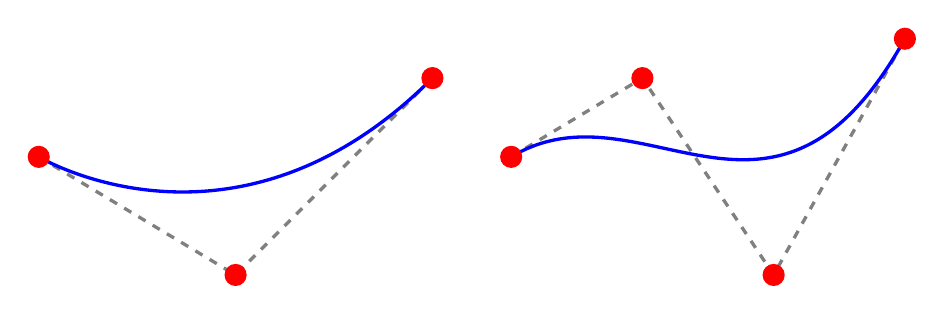
\begin{tikzpicture}[scale=5]
        \begin{scope}
            % Define the three control points
            \coordinate (P0) at (0,0.6);
            \coordinate (P1) at (0.5,0.3);
            \coordinate (P2) at (1,0.8);

            % Draw control polygon
            \draw[dashed, gray, very thick] (P0) -- (P1) -- (P2);
            \draw[blue, very thick] (P0) .. controls (P0) and (P1) .. (P2);

            % Draw and label the control points
            \foreach \pt in {(P0), (P1), (P2)} {
                \fill[red] \pt circle (0.8pt);
            }
        \end{scope}

        \begin{scope}[xshift=1.2cm]
            % Define the three control points
            \coordinate (P0) at (0,0.2+0.4);
            \coordinate (P1) at (1/3,0.4+0.4);
            \coordinate (P2) at (2/3,-0.1+0.4);
            \coordinate (P3) at (1, 0.5+0.4);

            % Draw control polygon
            \draw[dashed, gray, very thick] (P0) -- (P1) -- (P2) -- (P3);
            \draw[blue, very thick] (P0) .. controls (P1) and (P2) .. (P3);

            % Draw and label the control points
            \foreach \pt in {(P0), (P1), (P2), (P3)} {
                \fill[red] \pt circle (0.8pt);
            }
        \end{scope}
    \end{tikzpicture}
    \caption{BB-polynomials of degree two and three. (Approximate, the quadratic one is wrong.)}
\end{figure}

The derivative of a BB polynomial is given by
\begin{align*}
    p'(x)
    &= \sum_{i = 0}^d c_i (B_i^d)'(x) \\
    &= d \sum_{i = 0}^d c_i (B_{i - 1}^{d - 1}(x) - B_{i}^{d - 1}(x)) \\
    &= d \sum_{i = 0}^d c_i B_{i - 1}^{d - 1}(x) - d \sum_{i = 0}^d c_i B_{i}^{d - 1}(x) \\
    &= d \sum_{i = -1}^{d-1} c_{i+1} B_{i}^{d - 1}(x) - d \sum_{i = 0}^{d - 1} c_i B_{i}^{d - 1}(x) \\
    &= d \sum_{i = 0}^{d-1} c_{i+1} B_{i}^{d - 1}(x) - d \sum_{i = 0}^{d - 1} c_i B_{i}^{d - 1}(x) \\
    &= d \sum_{i = 0}^{d-1} (c_{i+1} - c_i) B_{i}^{d - 1}(x)
\end{align*}
such that
\begin{equation}
    p'(0) = d (c_1 - c_0).
\end{equation}
The slope between the first two control points is given by
\begin{equation}
    \frac{y_1 - y_0}{x_1 - x_0} = \frac{c_1 - c_0}{\frac{1}{d} - \frac{0}{d}} = d(c_1 - c_0),
\end{equation}
and we see that they match.
Again, the same property holds at the other end.
We write the derivative compactly as
\begin{equation}
    p'(x) = d \sum_{i = 0}^{d-1} \Delta c_i B_{i}^{d - 1}(x),
\end{equation}
with $\Delta c_i = c_{i+1} - c_i$.

This generalizes to higher order derivatives, with
\begin{equation}
    p^{(r)}(x) = \frac{d!}{(d - r)!} \sum_{i = 0}^{d - r} \Delta^r c_i B_i^{d-r}(x),
\end{equation}
where $\Delta^r c_i$ is the $r$-th order forward difference, defined by
\begin{equation}
    \Delta^r c_i = \Delta^{r - 1} c_{i + 1} - \Delta^{r-1} c_i.
\end{equation}

Integrating a BB polynomial is now easy, with the result from Bernstein polynomials at hand.
We have
\begin{equation}
    \int_{0}^{1} p(x) \, dx
    = \int_{0}^{1} \sum_{i = 0}^{d} c_i B_i^d(x) \, dx
    = \sum_{i = 0}^{d} c_i \int_{0}^{1} B_i^d(x) \, dx
    = \frac{\sum_{i = 0}^{d} c_i}{d + 1},
\end{equation}
which in other words is just the average of the coefficients.

\subsection{The de Casteljau algorithm}
The de Castljau algorithm gives an efficient way to evaluate a BB polynomial at a point.
We could use the recursion formula found previously, however we can instead recurse on the coefficients.
The algorithm is as follows:
\begin{enumerate}
    \item Set $c_i^0 = c_i$ for $i = 0, \dots, d$.
    \item For $r = 1, \dots, d$, compute $c_i^r = (1 - x)c_i^{r - 1} + x c_{i+1}^{r - 1}$ for $i = 0, \dots, d - r$.
    \item The final value $c_0^r$ is the value $p(x)$.
\end{enumerate}
To see why the final value is correct, note that by the recursion
\begin{align*}
    p(x)
    &= \sum_{i = 0}^{d} c_i B_i^d(x) \\
    &= \sum_{i = 0}^d c_i^0 (x B_{i-1}^{d-1}(x) + (1 - x)B_i^{d - 1}(x)) \\
    &= \sum_{i = 0}^d c_i^0 x B_{i-1}^{d-1}(x) + \sum_{i = 0}^{d} c_i^0 (1 - x)B_i^{d - 1}(x) \\
    &= \sum_{i = 0}^{d - 1} c_{i + 1} x B_{i}^{d - 1} + \sum_{i = 0}^{d - 1} c_i^0 (1 - x) B_i^{d - 1} \\
    &= \sum_{i = 0}^{d - 1} c_i^1 B_i^{d-1}.
\end{align*}
Continuing with this recursion, we end up with
\begin{equation}
    p(x) = \sum_{i = 0}^{0} c_i^d B_i^0 = c_0^d,
\end{equation}
as desired.

\subsection{BB splines}
In order to model complex functions with polynomials, we would typically have to have very high degree polynomials, which is not ideal.
What we do instead is utilize piecewise polynomial functions, called splines.
We will firstly do this with BB polynomial pieces, and in order to do that we need to amend a detail.

So far, we've only considered BB polynomials on the unit interval $[0, 1]$, but we now wish to do so on an arbitrary interval $[a, b]$.
The conversion is rather simple, as by writing
\begin{equation}
    x = (1 - \lambda) a + \lambda b,
\end{equation}
we get the mapping
\begin{equation}
    \lambda(x) = \frac{x - a}{b - a},
\end{equation}
such that $\lambda(x) \in [0, 1]$ for $x \in [a, b]$.
The only real difference we have now is that a BB polynomial
\begin{equation}
    p(x) = \sum_{i = 0}^{d} c_i B_i^d(\lambda)
\end{equation}
has control points $(\xi_i, c_i)$, with $\xi_i = \frac{d - i}{d} a + \frac{i}{d} b$.

Everything else is practically indentical, although we have to be careful to note that we require the chain rule when taking derivatives, as we need to compute
\begin{equation}
    \frac{d B_i^d(\lambda)}{dx} = \frac{d B_i^d(\lambda)}{d\lambda} \frac{d\lambda}{dx} = \frac{1}{b - a} \frac{d B_i^d(\lambda)}{d\lambda}
\end{equation}

Suppose we want to construct a spline $s$ defined by two polynomial pieces $p$ and $q$ on consecutive intervals $[a, b]$ and $[b, c]$, by
\begin{equation}
    s(x) =
    \begin{cases}
        p(x), & a \leq x < b, \\
        q(x), & b \leq x < c.
    \end{cases}
\end{equation}
Note that we've defined the spline to be left continuous.
We represent both $p$ and $q$ by BB polynomials, with
\begin{equation}
    p(x) = \sum_{i = 0}^{d} c_i B_i^d(\lambda)
    \quad\text{and}\quad
    q(x) = \sum_{i = 0}^{d} e_i B_i^d(\mu),
\end{equation}
where $\lambda$ and $\mu$ are the local coordinates for each interval.

The question then is how continuous we want this spline to be at the $s(b)$.
If we only want continuity, we have by the end point property that we need $c_d = e_0$, a relatively simple condition.
More generally, for $C^r$ continuity, we require that
\begin{equation}
    p^{(k)}(b) = q^{(k)}(b)
    \qquad
    k = 0, 1, \dots, r.
\end{equation}
Writing out these expressions we have
\begin{align*}
    \frac{d!}{(d - k)!} \frac{1}{(b - a)^k} \Delta^k c_{d-r} &= \frac{d!}{(d - k)!} \frac{1}{(c - b)^k} \Delta^k e_{0} \\
    \frac{1}{(b - a)^k} \Delta^k c_{d-r} &= \frac{1}{(c - b)^k} \Delta^k e_{0}
\end{align*}
as our condition.
Say for instance that we have the $c_i$ coefficients at hand, and wish to choose the $e_i$ coefficients such that we have $C^r$ continuity at the knot.
We can then choose
\begin{equation}
    e_i = \sum_{j = 0}^{i} c_{d - i + j} B_j^i(\alpha)
    \qquad i = 0, \dots, r,
\end{equation}
where $\alpha = \frac{c - a}{b - a}$.
I won't promise to remember the specifics of this\dots

\subsection{Spline interpolation}
Say we have some data, and we wish to fit a function to this.
How should we proceed?

\subsubsection{Linear spline interpolation}
Linear spline interpolation is perhaps the simplest.
Here, we have $x_1, x_2, \dots, x_m \in \mathbb{R}$ and associated values $y_1, y_2, \dots, y_m \in \mathbb{R}$., and wish to find a linear spline $g : [x_1, x_m] \to \mathbb{R}$ such that
\begin{equation}
    g(x_i) = y_i, \qquad i = 1, 2, \dots, m.
\end{equation}
We can do this simply by setting
\begin{equation}
    g_i(x) = y_i \frac{x_{i + 1} - x}{x_{i + 1} - x} + y_{i + 1} \frac{x - x_i}{x_{i + 1} - x_i},
\end{equation}
and having $g(x) = g_i(x)$ for $x_i \in [x_i, x_{i + 1}]$.
We can just as easily use BB polynomials, with
\begin{equation}
    g_i(x) = y_i B_0^1(\lambda_i) + y_{i + 1} B_1^1(\lambda_i).
\end{equation}

\subsubsection{Cubic Hermite spline interpolation}
If we use higher degree polynomial pieces, we are able to get a smoother spline.
We now let the $g_i$ segments be cubic polynomials, and we now have slope values $s_1, s_2, \dots, s_m$ in addition to the values previously, and we want to find $g$ such that
\begin{equation}
    g(x_i) = y_i
    \quad\text{and}\quad
    g'(x_i) = s_i,
    \qquad i = 1, 2, \dots, m.
\end{equation}
In the cubic case, we resolve this by setting
\begin{equation}
    g_i(x) = \sum_{j = 0}^{3} c_j B_j^3(\lambda_i(x)),
\end{equation}
with
\begin{equation}
    c_0 = y_i
    \qquad
    c_1 = y_i + \frac{h_i}{3} s_i
    \qquad
    c_2 = y_{i + 1} - \frac{h_i}{3} s_i
    \qquad
    c_3 = y_{i + 1}.
\end{equation}

\subsubsection{\texorpdfstring{$C^2$}{C2} cubic spline interpolation}
In order achieve a $C^2$ continuous cubic spline, we have a couple of options.
Here, we wish to find $g \in C^2[x_1, x_m]$ such that $g(x_i) = y_i$ for $i = 1, 2, \dots, m$, while additionally requiring
\begin{equation}
    g'(x_1) = s_1
    \quad\text{and}\quad
    g'(x_m) = s_m.
\end{equation}
One way to do this is to let $g$ be the Hermite interpolant from the previous section, and solving for the slopes $s_i$ such that
\begin{equation}
    g_i''(x_{i+1}) = g_{i + 1}''(x_{i + 1}).
\end{equation}
Let
\begin{equation}
    g_i = \sum_{j = 0}^{3} c_i B_j^3(\lambda_i)
    \quad\text{and}\quad
    g_{i + 1} = \sum_{j = 0}^{3} e_i B_j^3(\lambda_{i + 1}).
\end{equation}
Then,
\begin{align*}
    g_i''(x_{i + 1}) &= \frac{6}{h_i^2} (c_1 - 2 c_2 + c_3)
    = \frac{6}{h_{i}} \left(-\frac{y_{i} - y_{i + 1}}{h_i} \frac{s_i + 2 s_{i + 1}}{3}\right), \\
    g_{i + 1}''(x_{i + 1}) &= \frac{6}{h_{i + 1}^2} (e_0 - 2 e_1 + e_2)
    = \frac{6}{h_{i + 1}} \left(\frac{y_{i + 1} - y_{i + 2}}{h_{i + 1}} - \frac{2s_{i + 1} - s_{i + 2}}{3}\right).
\end{align*}
Equating the two gives us
\begin{equation}
    \alpha_i s_{i - 1} + 2 s_i + \beta s_{i + 1} = b_i
\end{equation}
with
\begin{equation}
    \alpha_i = \frac{h_i}{h_{i - 1} + h_i}
    \quad\text{and}\quad
    \beta_i = \frac{h_{i-1}}{h_{i - 1} + h_{i}},
\end{equation}
and
\begin{equation}
    b_i = \frac{3}{h_{i - 1} + h_i} \left(
        h_i \frac{y_i - y_{i - 1}}{h_{i - 1}}
        + h_{i - 1} \frac{y_{i + 1} - y_i}{h_i}
    \right).
\end{equation}
This results in the linear system
\begin{equation}
    \begin{bmatrix}
        2 & \beta_2 \\
        \alpha_3 & 2 & \beta_3 \\
        & \ddots & \ddots & \ddots \\
        && \alpha_{m - 2} & 2 & \beta_{m - 2} \\
        &&& \alpha_{m - 1} & 2
    \end{bmatrix}
    \begin{bmatrix}
        s_2 \\ s_3 \\ \vdots \\ s_{m - 2} \\ s_{m - 1}
    \end{bmatrix}
    =
    \begin{bmatrix}
        b_2 - \alpha_2 s_1 \\
        b_3 \\
        \vdots \\
        b_{m - 2} \\
        b_{m - 1} - \beta_{m - 1} s_m
    \end{bmatrix}.
\end{equation}

\subsubsection{Natural end conditions}
In the previous section, we required knowledge about the slopes at the end points in order to get anywhere.
And alternative to this is to apply \textit{natural end conditions}, where we set
\begin{equation}
    g''(x_1) = 0
    \quad\text{and}\quad
    g''(x_m) = 0.
\end{equation}
% Requiring $C^2$ continuity at the interior points $x_2, \dots, x_{m-1}$ gives us $m - 2$ equations, for which we have
This leads to the system
\begin{equation}
    \begin{bmatrix}
        2 & 1 \\
        \alpha_2 & 2 & \beta_2 \\
        & \ddots & \ddots & \ddots \\
        && \alpha_{m-1} & 2 & \beta_{m - 1} \\
        &&& 1 & 2
    \end{bmatrix}
    \begin{bmatrix}
        s_1 \\ s_2 \\ \vdots \\ s_{m - 1} \\ s_m
    \end{bmatrix}
    =
    \begin{bmatrix}
        b_1 \\ b_2 \\ \vdots \\ b_{m - 1} \\ b_m
    \end{bmatrix},
\end{equation}
with
\begin{equation}
    b_{1} = 3\frac{y_2 - y_1}{h_1}
    \quad\text{and}\quad
    b_m = 3 \frac{y_m - y_{m - 1}}{h_{m - 1}}.
\end{equation}

\section{B-Splines}
A B-spline is defined from a set of knots
\begin{equation}
    \boldsymbol{t} = (t_1, t_2, \dots, t_{n + d + 1}),
\end{equation}
where $n$ and $d$ are respectively the number and degree of the B-splines.
We assume that the knotvector satisfies
\begin{equation}
    t_{i} \leq t_{i + 1}
    \quad\text{and}\quad
    t_{i} < t_{i + d + 1}.
\end{equation}
The $i$-th B-spline is then defined by
\begin{equation}
    B_{i, d, \boldsymbol{t}}(x)
    = B[t_i, t_{i + 1}, \dots, t_{i + d + 1}](x)
    = [t_i, t_{i + 1}, \dots, t_{i + d + 1}](\cdot - x)_+^d,
\end{equation}
where we here use the divided differences of the truncated power.

B-splines satisfy the property that $B_{i, d, \boldsymbol{t}}(x)$ is zero for all $x \notin [t_i, t_{i + d + 1}]$.
We can see this simply for $x > t_{i + d + 1}$, as then
\begin{equation}
    (t_j - x)_+^d = 0,
    \qquad
    j = i, i + 1, \dots, i + d + 1.
\end{equation}
In the other case, where $x < t_i$, we need an important result for divided differences.
One definition for divided differences is that for a function $f$ defined at points $x_0, x_1, \dots, x_k$, the divided difference of $f$ is the leading coefficient in monomial form of the interpolating polynomial.
Importantly in our case, for $x < t_i$, we have that
\begin{equation}
    (t_j - x)_+^d = (t_j - x)^d \in \pi_d
    \qquad
    j = i, i + 1, \dots, i + d + 1.
\end{equation}
Of important note is that we have $d + 2$ points, such that the interpolating polynomial has a zero coefficient in the leading term.

We also have translation invariance of the B-splines, i.e.\ that
\begin{equation}
    B[t_i + y, t_{i + 1} + y, \dots, t_{i + d + 1} + y](x)
    = B[t_i, t_{i + 1}, \dots, t_{i + d + 1}](x - y).
\end{equation}
We can see this as
\begin{equation}
    ((t + y) - x)_+^d = (t - (x - y))_+^d.
\end{equation}

In the simples case, where $d = 0$, we have
\begin{equation}
    B_i,0(x) = -(t_i - x)_+^d + (t_{i + 1} - x)_+^d,
\end{equation}
showing clearly that the $B_{i, 0}$ is only non-zero on the interval $[t_i, t_{i + 1}]$, where it is equal to one.

In the case of an arbitrary function $f$, we that
\begin{equation}
    [x_0, x_1, \dots, x_{k}]f
    = \sum_{i = 0}^{k} \frac{
        f(x_i)
    }{
        \prod_{\substack{j = 0 \\ j \neq i}}^{k} (x_i - x_j)
    }.
\end{equation}
This allows us to write explicitly
\begin{equation}
    B_{i, d}(x) = \sum_{j = i}^{i + d + 1} a_j (t_j - x)_+^d,
\end{equation}
with
\begin{equation}
    a_j = \frac{t_{i + d + 1} - t_i}{\prod_{\substack{k = i \\ j \neq i}}^{i + d + 1} (t_j - t_k)}.
\end{equation}

\end{document} % chktex 17